\documentclass{report}
\usepackage{tipa}
\usepackage{lmodern}
\usepackage{multirow}
\usepackage{amssymb}
\usepackage[table,xcdraw]{xcolor}
\usepackage{listings}
\usepackage{tikz}
\usepackage{tikz-qtree}
\usepackage{url}
\usepackage{graphicx}
\usepackage{todonotes}
\usepackage{tcolorbox}
\usepackage{algorithm}
\usepackage{algpseudocode}
\usepackage[backend=biber,style=numeric,sorting=none]{biblatex}
\usepackage{fontspec}
\usepackage{gb4e}

\setcounter{biburllcpenalty}{7000}
\setcounter{biburlucpenalty}{8000}

\lstset{basicstyle=\ttfamily}

\newfontface\lserif{Consolas}
\newcommand{\Csh}{C{\lserif\#}}

\fontsize{11pt}{1.2}


\definecolor{lightgray}{HTML}{EEEEEE}

\addbibresource{bibliography.bib}

\title{Creating a library to aid in constructed language generation}
\author{Daniel James}
\date{April 2017}
\begin{document}% %
   \maketitle
   
   \chapter{Introduction}
   \textit{yod} is a library, written in \Csh{}, designed to aid in the construction and generation of artificial languages. Artificial languages (also known as constructed languages or `conlangs') are probably most publicly well known through the popularisation of `fictional languages' - that is, languages designed for use in works of fiction, usually for adding depth to a fictional world. For example, J. R. R. Tolkien devised the languages of \textit{Sindarin} and \textit{Quenya} for use in his \textit{Lord of the Rings} series. Other popular fictional languages that have reached mainstream awareness include \textit{Star Trek}'s \textit{Klingon} and \textit{Game of Thrones}' \textit{Dothraki}.
   
   The creation of these languages has become an indispensable tool for writers to add depth and character to their worlds. However, constructed languages do not exist solely for creative uses. The language \textit{Esperanto} was developed by its creator L. L. Zamenhof with the goal of being a global language that was easy for people to learn\cite{unualibro}. Now it is reported that as many as 63,000 people worldwide can speak Esperanto to some degree\cite{esperanto}. The existence of Esperanto and other so-called `international auxiliary languages' (languages designed to simplify complication between people of different countries and cultures) shows that the usefulness of constructed languages extends into real-world applications as well as artistic uses.
   
   \textit{yod} was developed with a focus on artistic languages, and so the goal was to generate a large variety of languages which could suit many different worlds and fictional civilisations. However, due to the hierarchy of rules \textit{yod} uses to build languages, the languages are regular, in contrast to most natural languages, which means generated languages with certain features could be treated as auxiliary languages too.
   
   As a library, \textit{yod} provides interfaces to easily generate any part of a language, including phonology, orthography and grammar and sub-parts thereof. This works by having each class which represents a randomisable constituent exposing a \texttt{Generate()} method which creates a new instance of that class from scratch with procedurally generated properties. If necessary, this sometimes also means recursively generating that objects constituent members. Writing these generator methods in a way that takes into account certain restrictions or statistics allows for much more realistic values for the object.
   
   Merely generating a new language every time the library is used, however, would not allow for enough control over the language generation process for users who are more experienced with the concept of `conlangs' and the construction thereof. It also does not allow for iterative language-building, wherein the user keeps features of a generated language that they like, but re-generates the rest of the features. This would allow a user to quickly and easily refine their language until it suited their use case.
   
   To facilitate this, \textit{yod} uses a data-driven approach which allows almost every class that can be randomly generated to also be serialised to and deserialised from external data files. These data files are written in JSON to allow for them to be altered or loaded by other tools, or if necessary, by hand. Provided is a basic command line interface to the library which can handle almost every step of the generation process. This is a simple example of a tool which can load and create the data files produced by the library, and utilise the library's API. Providing the language-generation tools as a library allow for more complex tools to grow which implement and interact with the code.
   
   The library format also allows for software which might have a need for `conlangs' to generate them directly and use them immediately, as opposed to generating one and then using the output files as input for the program. One such example could be in the case of a video game which requires a cohesive strategy for naming places, characters, flavour text etc. These entities could have their text generated on the fly, without any input from the game developer or writers. The \textit{yod} library also allows the random number generator (which provides random values for all of the rest of the code) to be given a seed, meaning it will produce the same output every time. Thus, the objects in the aforementioned game could have different text every time the game was run, or the developer could choose a seed that gave output that suited them and keep that the same, without having to copy text from the output of the script into the game's script and data files.
   
   \todo{talk about structure}
   
   \chapter{Phonology}
   The `na\"{\i}ve' method of building words is by taking an alphabet (for example, the Latin alphabet) and concatenating random characters until the sequence reaches a random length between a minimum and maximum. For example, given $min = 3$ and $max = 8$ the following example text can be generated.
   
   \begin{figure}[h]
   \caption{Random letters from the Latin alphabet}
   \label{random letters from latin alphabet}  
   \begin{tcolorbox}
\texttt{tqk qzsyjla msmnix jvxx wug sysrh cuepg snyow ptjo bcek arjdubw pfwpt nabgzk jmq taphh zewll dmpr uvpmx sfpfk uuo bdm vnjbq hahuj wstq kohvma irn fott axdut rlgg tawz wsol wigom psqwd tnv vlzgt lbcikk bof msmyg zkqgubb veht ukaznqn ixp rppfj eqllnko uyyp aot uowtn icv fgypx cenawnk hypq rruh eosgrf wmakeg hhweua gnbfh mkpzi ebtwbv cjwrxw ucky kqezcm ucme wmrk khsya llzbeqw uxwivpp pbao gkzu pda txdp iwl gkmfqn uxeupe atjxy vyul}
   \end{tcolorbox}
\end{figure}
   
   Several problems can be immediately seen with this generated text. First, many of the words are difficult to pronounce and unrealistic with regards to their consonant clusters - for example, words like \verb|jvxx| and \verb|rppfj| are unlikely to exist in any natural languages. Generating words in this manner will also not produce very much variation in languages, as each letter has an equal probability to be picked.
   
   We also quickly run into the problem of representing language in text. \todo{cite}Written languages are based on spoken languages, so generating a written language first without basing it on a spoken one will lead to an unrealistic language. Furthermore, it is hard to say how our generated words are pronounced - one can apply English pronunciations to some of the words (for example \verb|tawz| becomes \textipa{/tO:z/} and \verb|axdut| becomes \textipa{/"\ae ks.d2t/}), but this results in a very Anglo-centric phonology, as we are biased to only use phonemes that exist in our own language while pronouncing unknown words.
   
   Because of these problems, it is obvious that merely stringing together random characters with no thought towards pronunciation is insufficient when it comes to creating realistic and varied languages. Therefore it is necessary to first create a phonology on which to base all of our language's words.
   
   \section{Phonetic inventory}
   
   In its simplest form, a phonology is a list of every sound that is included in a language. \todo{cite (WALS)}English phonology, for example, contains around 24 consonants (with more or less depending on dialect) and anywhere between 7 and 14 vowels, again depending heavily on dialect. The phonology for the `Received Pronunciation' dialect of English can be seen in \ref{english consonants} and \ref{english vowels}.
   
  \begin{table}[h]
  	\caption{Consonant inventory in English phonology}
  	\label{english consonants}
  	\centering
  	\makebox[0pt]{
	  	\begin{tabular}{|
	  			>{\columncolor[HTML]{D8D8D8}} l |
	  			>{\columncolor[HTML]{D8D8D8}} l |llllll}
	  		\hline
	  		\textbf{} & \textbf{} & \cellcolor[HTML]{D8D8D8}\textbf{Labial} & \cellcolor[HTML]{D8D8D8}\textbf{\begin{tabular}[c]{@{}l@{}}Dental,\\ Alveolar\end{tabular}} & \cellcolor[HTML]{D8D8D8}\textbf{Post-alveolar} & \cellcolor[HTML]{D8D8D8}\textbf{Palatal} & \multicolumn{1}{l|}{\cellcolor[HTML]{D8D8D8}\textbf{Velar}} & \multicolumn{1}{l|}{\cellcolor[HTML]{D8D8D8}\textbf{Glottal}} \\ \hline
	  		\textbf{Nasal} & \cellcolor[HTML]{D8D8D8} & \textipa{m} & \textipa{n} &  &  & \textipa{N} &  \\ \cline{1-1}
	  		\textbf{\begin{tabular}[c]{@{}l@{}}Plosive,\\ Affricate\end{tabular}} & \multirow{-2}{*}{\cellcolor[HTML]{D8D8D8}} & \textipa{p} / \textipa{b} & \textipa{t} / \textipa{d} & \textipa{\t{tS}} / \textipa{\t{dZ}} &  & \textipa{k} / \textipa{g} &  \\ \cline{1-2}
	  		\cellcolor[HTML]{D8D8D8} & \textbf{Sibilant} &  & \textipa{s} / \textipa{z} & \textipa{S} / \textipa{Z} &  &  &  \\ \cline{2-2}
	  		\multirow{-2}{*}{\cellcolor[HTML]{D8D8D8}\textbf{Fricative}} & \textbf{Non-sibilant} & \textipa{f} / \textipa{v} & \textipa{T} / \textipa{D} &  &  & \textipa{x} & \textipa{h} \\ \cline{1-2}
	  		\textbf{Approximant} & \textbf{} &  & \textipa{l} & \textipa{r} & \textipa{j} & \textipa{w} &  \\ \hline
	  	\end{tabular}
  	}
  \end{table}

	\begin{table}[h]
		\centering
		\caption{Vowel inventory in English phonology (Received Pronunciation)}
		\label{english vowels}
		\begin{tabular}{|
				>{\columncolor[HTML]{D8D8D8}}l |lll}
			\hline
			& \multicolumn{1}{l|}{\cellcolor[HTML]{D8D8D8}Front} & \multicolumn{1}{l|}{\cellcolor[HTML]{D8D8D8}Central} & \multicolumn{1}{l|}{\cellcolor[HTML]{D8D8D8}Back} \\ \hline
			Close & \textipa{i} / \textipa{I}                                              &                                                      & \textipa{u} / \textipa{U}                                        \\ \cline{1-1}
			Mid   & \textipa{e}                                                  & \textipa{3} / \textipa{@}                                            & \textipa{O}                                        \\ \cline{1-1}
			Open  & \textipa{\ae}                                                 & \textipa{2}                                         & \textipa{A} / \textipa{6}                                    \\ \cline{1-1}
		\end{tabular}
	\end{table}

	Other languages have different phonemic inventories, with varying numbers of consonants and vowels. Some, for example, have as few as 3 vowels, or as many as 84 or more consonants, depending on the method of counting\cite{leverbeoubykh}. A very large factor in the variety of languages generated is the phonology, as it restricts the type of sounds which often has a profound impact on how it is perceived. Therefore the first step towards a completed language should be a randomly generated, unique phonology.
	
	The International Phonetic Alphabet (IPA) is an alphabet created by the International Phonetic Association for phonetic representation of speech and language\cite{ipahandbook}. It contains (or aims to contain) distinct symbols for each unique sound possible to create that is part of a language. As such, it provides a perfect way to convey the `end result' of generation process, since it can describe precisely how every word in the language is pronounced. The IPA also includes markers for syllable stress and other important factors which can be included in speech. In order to avoid the user from having to infer the pronunciation of a word from its orthography (how it is written), \textit{yod} can produce an IPA transcription of its output, which shows exactly how to pronounce it without ambiguity.
	
	However, the IPA can also be used as a basis for \textit{creating} a phonology. It lists every sound possible in a language, so as a na\"{\i}ve approach would be to randomly choose sounds from this set to build words. This approach is similar to the approach which was taken before, which involved choosing random letters from the Latin alphabet. However this time the words are being generated via sound directly rather than generating a written word, then trying to create a spoken representation of that.
	
	The problems with taking the entire IPA as our set of possible sounds are twofold. First, it does not give us a unique phonology - instead the phonology is the same every single time, as its contents are not randomised. Second, if the phonology for the generated language contains \textit{every} consonant and vowel from the IPA, then it will have many more phonemes than even the largest existing phonetic inventory. This is clearly unrealistic, and would be very difficult for anybody to learn. For artistic languages, this is a bit less of a concern but it is still preferable that the generated words be somewhat pronounceable and understandable, which gets less likely the more phonemes a speaker would have to discern from each other.
	
	To create more realistic phonologies, the subset of sounds taken from the full phonetic alphabet can be restricted. If, for example, random phonemes from the set are formed into words of random length between 3 and 8, the following words could be produced:
	
	\begin{figure}[h]
	\caption{Random subset of all phonemes}
	\label{random subset of all phonemes}	
	\begin{tcolorbox}
		\texttt{
			\textipa{\:lTT\textraising{\={\*r}} \c{c}g\t{dz} e\t{dz}\:R\:lV \:l\t{\=*{\r*t}\textraising{\={\*r}}}g\t{\=*{\r*t}\textraising{\={\*r}}}XU\:R\t{\=*{\r*t}\textraising{\={\*r}}} \:l\textraising{L}\r*g\textraising{\={\*r}}\c{c} \t{dz}\textcrh\t{\:d\:z} \textcrh\textcrh\r*{\:R}\textraising{\={\*r}}eT e\t{dz}\c{c}\t{dz} \r*LV\t{dz}e\:lV U\:lUX\textcrh}
		}
	\end{tcolorbox}
	\end{figure}

	Although this method achieves variety of phonemes while keeping the total number of phonemes low - the phonology used to generate these words only contains 15 phonemes - a lot of the words are still unrealistic. Similar to figure \ref{random letters from latin alphabet}, there are an abundance of large consonant clusters. Most words in the output lack a vowel and even those with vowels have extremely unrealistic consonant clusters.
	
	Another problem with this generated output is the sequences \textipa{/TT/} and \textipa{/\textcrh\textcrh/}. The former contains adjacent voiceless dental fricatives, and the latter contains adjacent voiceless pharyngeal fricatives. Such sequences consisting of two of the same phonemes are unpronounceable and would most likely be realised as single instances of the phoneme (e.g. \textipa{/T/} and \textipa{/\textcrh/}). These problems show that this method of generation is still insufficiently realistic.
	
	Is is important now to separate the phonology somewhat from the process of creating words. The problems just discussed are largely more to do with this word creation process, whereas there is still some work to do to improve the selection of individual phonemes for the phonology.
	
	The first step is to create a distinction between the two different types of phonemes: consonants and vowels. Consonants and vowels have very different features, and play very different roles in the formation of words. Thus the phonology's set of consonants should be generated separately from its set of vowels.
	
	Both consonants and vowels share the common features of phonemes shown in figure \ref{shared properties of phonemes}. Sonority is a numerical representation of how loud or sonorous the phoneme. Each phoneme also has a representative symbol in the International Phonetic Alphabet so they can be easily transcribed.
	
	\begin{figure}
		\caption{Shared properties of phonemes}
		\label{shared properties of phonemes}
		\begin{tcolorbox}
			\begin{itemize}
				\item IPA symbol representation
				\item Sonority
			\end{itemize}
		\end{tcolorbox}
	\end{figure}

	In addition to these shared properties, consonants also have the extra features shown in figure \ref{properties of consonants}.
	
	\begin{figure}[h]
		\caption{Unique properties of consonants}
		\label{properties of consonants}
		\begin{tcolorbox}
			\begin{itemize}
				\item Place of articulation
				\item Manner of articulation
				\item Phonation/Voicing
				\item Gemination
			\end{itemize}
		\end{tcolorbox}
	\end{figure}
	
	The place of articulation refers to the part of the vocal track that creates an obstruction of airflow. The manner of articulation describes \textit{how} this obstruction affects the airflow - for example, `stops' or `plosives' completely block airflow, whereas `sibilants' and `fricatives' merely result in a turbulent airflow. The phonation of a consonant refers to whether, in producing the sound, the larynx affects the airflow through vibration of the vocal folds. Geminate consonants are consonants which are pronounced for a longer period of time, contrasting the usual shorter consonants. In `stops' this is realised as a delayed release of the consonant, whereas other consonants with other types of articulation are merely prolonged.
	
	Similarly to consonants, vowels can be distinguished by the features in figure \ref{properties of vowels}.
	
	\begin{figure}[h]
		\caption{Unique properties of vowels}
		\label{properties of vowels}
		\begin{tcolorbox}
			\begin{enumerate}
				\item Height
				\item Backness
				\item Roundedness
				\item Length
			\end{enumerate}
		\end{tcolorbox}
	\end{figure}

	A vowels characteristics are formed from the position of the tongue in the mouth and the rounding of the lips. The height of a vowel refers to the height of the tongue, and the backness is the forward/back position of the tongue. Roundedness is the state of the lips in pronouncing the vowel - either rounded or unrounded. This unrounded/rounded distinction can be seen in the difference between the two open mid-back vowels \textipa{/2/} and \textipa{/O/} (compare \textit{shut} \textipa{/S2t/} and \textit{short} \textipa{/SO:t/}). The word \textit{short} \textipa{/SO:t/} also shows a good example of a long vowel (although there is no long/short vowel distinction in most English dialects\todo{cite?}).
	
	In fact, both height and backness are defined by the formant frequency of the voice, which are produced by the tongue's position. A spoken vowel can be represented with two formants \textit{F1 = height} and \textit{F2 = backness}. Roundness also has an effect on these formants, usually being seen as a decrease in \textit{F2} as well as a small decrease in \textit{F1}.
	
	It can be seen that both vowels and consonants have properties which relate to their length; these being consonants' gemination and vowels' length. Due to the similarities between these properties, they can be abstracted into the set of base phoneme properties as a `Length' property. Thus the final set of properties ends up being as follows:

	\begin{figure}[h]
	\caption{Shared properties of phonemes, with length}
	\label{shared properties of phonemes with length}
	\begin{tcolorbox}
		\begin{itemize}
			\item IPA symbol representation
			\item Sonority
			\item Length
		\end{itemize}
	\end{tcolorbox}
	\end{figure}

	This arrangement of properties lends itself extremely well to a simple data structure in \Csh{}. Consonants and vowels both translate trivially to classes, with their respective properties existing as enum members in those classes. For example, an enum \texttt{PlaceOfArticulation} can be created to represent the place of articulation of a consonants which would contain the set of values \texttt{Bilabial}, \texttt{Labiodental}, \texttt{Lingulabial}, \texttt{Dental} etc. Both the \texttt{Consonant} and \texttt{Vowel} classes are subclasses of a more general, abstract \texttt{Phoneme} class which contains only the properties that are shared between both of them. This allows the entire International Phonetic alphabet to be represented in code as a set of \texttt{Phoneme}s.
	
	It is more useful, however, to distinguish between the set of vowels and the set of consonants. Thus the two classes \texttt{ConsonantCollection} and \texttt{VowelCollection} can act as lists of their respective type of phoneme, with a \texttt{PhonemeCollection} being formed out of a union of the two sets of phonemes. Each class's \texttt{Generate()} method can then be used to create a unique set of each type of phoneme.
	
	Using statistics from the World Atlas of Language Structures, the realism of our phonology generation can be increased by roughly following the range distribution of numbers of vowels and consonants in natural languages. For vowels, the distribution is shown in figure \ref{vowel quality inventories}. By using these numbers as weights for a weighted random algorithm, the vowel inventory in the generated phonology will be similar in size to natural languages' vowel inventories. The result of the weighted random algorithm is a range (minimum value and a maximum value). Using \textit{yod}'s global random number generator, a value between these maximum and minimum can be chosen as the goal number of vowels. Then that amount of unique vowel sounds can be randomly chosen from the full set to complete the vowel inventory.
	
	\begin{table}[]
		\centering
		\caption{Vowel Quality Inventories\cite{wals-2}}
		\label{vowel quality inventories}
		\begin{tabular}{|>{\columncolor[HTML]{D8D8D8}}l |l|}
			\hline
			Value	&	\cellcolor[HTML]{D8D8D8}Representation \\
			\hline
			Small vowel inventory (2-4)                                   & 93                                     \\ \hline
			Average vowel inventory (5-6)                                 & 287                                    \\ \hline
			Large vowel inventory (7-14)                                  & 184                                    \\ \hline \hline
			\multicolumn{1}{|r|}{\cellcolor[HTML]{D8D8D8}\textbf{Total:}} & 564                                    \\ \hline
		\end{tabular}
	\end{table}
	
	\begin{table}[]
		\centering
		\caption{Consonant Quality Inventories\cite{wals-1}}
		\label{consonant quality inventories}
		\begin{tabular}{|>{\columncolor[HTML]{D8D8D8}}l|l|}
			\hline
			Value                    & \cellcolor[HTML]{D8D8D8}Representation \\ 
			\hline
			Small (6-14)             & 89             \\
			Moderately small (15-18) & 122            \\
			Average (19-25)          & 201            \\
			Moderately large (26-33) & 94             \\
			Large (34 or more)       & 57             \\ \hline \hline
			\multicolumn{1}{|r|}{\cellcolor[HTML]{D8D8D8}\textbf{Total:}} & 563                                    \\ \hline
		\end{tabular}
	\end{table}

	Similarly, figure \ref{consonant quality inventories} shows the range distribution of consonants in natural languages. The same weighted random algorithm can be used to get a range, then a random `goal' value of consonants in that range.
	
	For consonants, however, it does not need to be as simple as choosing random consonants from the set of all consonants in the IPA. There are approaches that can be used to pick consonants in a smarter way which will result in better consonant inventories.
	
	Given a goal number of consonants that need to be added to the phonology, the aim is procedurally get as close to that number while taking into account extra statistics for which consonants to pick. Adding and removing whole places or manners of articulation tends to be more natural than choosing consonants at random\todo{cite - only thing i know about this is that one Artifexian video}, so a way of modelling this would be to add places and manners of articulation until the intersection of them results in the right amount of consonants. The algorithm would therefore work something like this:
	
	\begin{algorithm}
		\caption{Consonant inventory generation algorithm}
		\label{consonant inventory generation algorithm}
		\begin{algorithmic}[1]
		\State $goal \gets$ generated goal number of consonants
		\State $places \gets \varnothing $
		\State $manners \gets \varnothing $
		\State $consonants \gets \varnothing $
		\While{$\left\vert{consonants}\right\vert < goal$}
			\If{$random < 0.5$}
				\State $places \gets places \cup \{$random place of articulation$\}$
			\Else
				\State $manners \gets manners \cup \{$random manner of articulation$\}$
			\EndIf
			\State $consonants \gets \{x | x.place \in places \wedge x.manner \in manners\}$
		\EndWhile
		\end{algorithmic}
	\end{algorithm}

	Generating a consonant inventory this way means that the resulting language will be more cohesive in its sounds, while still retaining a unique feel every time one is generated. This approach does not take into account the phonation of consonants, though, so more variety could still be added. Again, WALS provides statistics on voicing in natural languages. Figure \ref{voicing in plosives and fricatives} shows the distribution of languages which have a distinction between voiced and unvoiced fricatives and plosives.
	
	\begin{table}[h]
		\centering
		\caption{Voicing in Plosives and Fricatives\cite{wals-4}}
		\label{voicing in plosives and fricatives}
		\begin{tabular}{|>{\columncolor[HTML]{D8D8D8}}l|l|}
			\hline
		    Value                                            & Representation \\ \hline
		No voicing contrast                              & 182            \\
		Voicing contrast in plosives alone               & 189            \\
		Voicing contrast in fricatives alone             & 38             \\
		Voicing contrast in both plosives and fricatives & 158            \\ \hline \hline
			\multicolumn{1}{|r|}{\cellcolor[HTML]{D8D8D8}\textbf{Total:}} & 567                                    \\ \hline
		\end{tabular}
	\end{table}

	The figure shows information about voicing in both fricatives and plosives. In order to get this information from the statistics into a form that can be used in code, the \textbf{Value} column can instead be seen as a tuple of two boolean values: `voicing contrast in plosives' and `voicing contrast in fricatives'. With an object structure of \verb|{fricative voicing contrast, plosive voicing contrast}| The values will then become \verb|{false, false}|, \verb|{false, true}|, \verb|{true, false}| and \verb|{true, true}|. By using a weighted random algorithm, as above, to choose a random tuple, the respective values can be taken from the tuple and set in our consonant-choosing code.
	
	These values do not refer to whether voiced or unvoiced phonemes themselves are included in the phonology - rather they describe whether there is a distinction made between voiced and unvoiced phonemes. This can be simplified as `if the language makes a distinction between the two, include both voicings.' Otherwise, the algorithm should only include only the consonant which has the phonology's `voicing' for that manner of articulation, which can be chosen randomly.
	
	By using these refinements for generating a phonetic inventory, a unique and varied, yet still realistic, phonology can begin to be generated. This phonology provides the basis upon which the rest of the language is built.

	\section{Syllables}
	
	The next step towards a full phonology is building syllables out of the phonemes from the generated phonetic inventory.
	
	\begin{figure}[h]
		\caption{Syllable structure}
		\label{syllable structure}
		\centering
		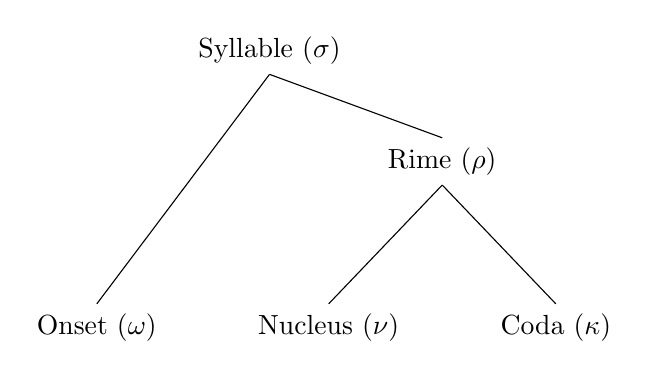
\begin{tikzpicture}				
			\tikzset{level distance=40pt}
			\tikzset{sibling distance=30pt}
			\tikzset{frontier/.style={distance from root=100pt}}
			\Tree [.{Syllable ($\sigma$)} {Onset ($\omega$)} [.{Rime ($\rho$)} {Nucleus ($\nu$)} {Coda ($\kappa$)} ] ]
		\end{tikzpicture}
	\end{figure}

	Figure \ref{syllable structure} shows the structure of a syllable. A syllable is formed out of two parts - the \textit{onset} and the \textit{rime}. Furthermore, the rime consists of a usually required \textit{nucleus} and a \textit{coda}. Both the onset and coda can be consonants or consonant clusters. The nucleus consists of a vowel or vowels (monophthong or diphthong).
	
	The role of \textit{yod} is to construct syllables that fit this structure and then form them into words. The simplest method of generating syllables is by taking random phonemes from the pre-generated phoneme inventory and filling the onset, nucleus and coda with them. This method can be easily refined by not always filling all the parts of the syllable - the onset and coda can both be optional, so adding them in every instance is less realistic.
	
	Another simple improvement that can be made is allowing for consonant clusters and diphthongs, which is done by picking multiple phonemes when filling a section. In order to vary the results, this should not be done every time, but should vary in frequency. The addition of clusters and diphthongs allows for more complex syllables to be created.
	
	The maximum number of consonants in a consonant cluster, the maximum number of vowels in the nucleus, as well as whether any of the parts of the syllable are optional, are all properties of the language. Thus, syllable structures can be generated. The structure of a syllable is commonly shown as a string of either `C's or `V's (consonants or vowels)\cite{clements1985cv}. A language permitting only syllables with exactly one onset consonant and exactly one vowel, and no coda, would be described as having a CV syllable structure.
	
	This representation also shows variable structures where some phonemes are optional - that is, the number of phonemes in a segment can differ. For this, bracket notation is used to denote an optional phoneme. For example, the syllable structure of the English language is cited as being (C)(C)(C)V(C)(C)(C)(C). This represents a syllable structure where the onset can have 0-3 consonants, the nucleus always contains a vowel, and the coda can have 0-4 consonants. While it is rare in English for a syllable to have the largest possible onset \textit{and} coda clusters at the same time, examples can still be seen; the monosyllabic word \textit{strengths} can be transcribed as \textipa{/st\*rENkTs/}. This word displays an onset cluster of length 3 (\textipa{/st\*r/}) and a coda cluster of length 4 (\textipa{/NkTs/}).
	
	In order to generate a syllable structure in its most basic form, a minimum and maximum cluster value can be defined for onset, nucleus and coda. This yields a decently varied set of possible structures. To augment this, weights can be assigned to each possible value from the minimum to maximum, meaning that some lengths of phoneme clusters will be rarer than others. As in the case of the English language's 4-length coda consonant cluster, which is uncommonly seen, some clusters in the generated language will be less common. Not only does this increase variety in the languages that \textit{yod} generates, but it also is more realistic, as it would be unusual to have all possible cluster lengths equally probable.
	
	Now, with a syllable structure for the language decided, a syllable can be created based on it. First, a syllable structure is needed for this syllable - this can be randomly generated from the phonology's structure. For example, given English's (C)(C)(C)V(C)(C)(C)(C) structure, there are many possible subsets of structures that a syllable could have and still be considered valid. At its most complex, a syllable could match the above structure exactly, and at its simplest the syllable could just have the structure V. Most syllables will lie somewhere inbetween these two extremes. Treating the onset, nucleus and coda separately, a random value can be selected using a weighted random algorithm on our weighted set of possible values. Then a number of phonemes equal to the chosen number for each section can be chosen. By concatenating the onset phonemes, the nucleus and the nucleus phonemes in that order, a syllable is created.
	
	Using this method, and the set of phonemes from the English phonology, the sample set of syllables in figure \ref{sample syllables with weighted structure} was generated. The syllables in the figure are based on a generated syllable structure of (C)(C)V(C)(C).
	
	\begin{figure}
		\caption{Sample syllables with weighted structure (C)(C)V(C)(C)}
		\label{sample syllables with weighted structure}  
		\begin{tcolorbox}
		\textipa{
			/\*rl6z Didg @pn vOsg \*ru SZUsT I Dj\ae{} t\ae{} s6w vz2f 6kk NOh eD \ae T ASZ 6sD fT3D 6Z SI \t{dZ}6p @h h@zw b@p Nujn Il giZw \ae Sh sjOl \t{dZ}\ae ND 2\t{dZ} v\ae{} TUlD iD\t{dZ} zAl nA vS3st 2f\t{dZ} lOwm \*rAl\t{dZ} \t{dZ}tU\t{dZ}d l3vz 3 6 idl 2jn pb6hm t\t{dZ}AfD f3Sj/
		}		
		\end{tcolorbox}
	\end{figure}

	Both syllables that match the most complex possible structure in this phonology (\textipa{/\t{dZ}tU\t{dZ}d/} and \textipa{/pb6hm/}) and the least complex possible structure (\textipa{/3/} and \textipa{/6/} can be seen in this selection, showing the range of the syllable generation code. If each syllable in this sample is considered to be a monosyllabic word, the results from this code are already noticeably more realistic than the words generated in figures \ref{random letters from latin alphabet} and \ref{random subset of all phonemes} (although in this sample only the phonemes from the English phonology are used, which can give a false sense of `realism'). The structure of building clusters of consonants around a central vowel base creates realistic syllables.
	
	However, there are still some instances where unrealistic phoneme sequences can be spotted, even in this short sample of results. For example, the initial cluster of \textipa{/pb/} in the word \textipa{/pb6hm/} consists of two successive stops - both the voiced and unvoiced bilabial plosive. For a word to contain multiple plosives in a row already makes it harder to pronounce, and the fact that they are both bilabial plosives only increases that difficult. Either both are audibly released, which results in a long, difficult to pronounce cluster, or the first consonant will be deleted completely\todo{cite}. The generated syllable \textipa{/6kk/} also provides some trouble, as `double consonants' are rare in IPA transcriptions of natural languages. Usually when a double consonant appears in a transcription, it will either be across a syllable boundary (e.g., a sequence \textipa{/\dots{}kk\dots{}/} is likely to represent the coda of one syllable and the onset of another syllable \textipa{/\dots{}k.k\dots{}/}) or the gemination of the consonant (e.g., \textipa{/\dots{}kk\dots{}/} is another way of writing \textipa{/\dots{}k:\dots{}/}). However, these uses are rare, and most commonly a single consonant would be used in their place, or the IPA symbol for gemination inserted.
	
	In order to solve the problem of unrealistic consonant clusters, syllables can be built based on a `sonority hierarchy'. The sonority hierarchy is a scale showing the relative strength of different phonemes based on their properties\cite{burquest2006}. Different phonemes have different amplitudes, and patterns in the amplitudes can be seen depending on the place and manner of articulation, as well as the phonation. It can be seen that syllables in many natural languages follow a structure whereby the nucleus has the most sonorant phonemes, and then the rest of the phonemes in the syllable decrease in sonority as they get further away from the nucleus. This is known as the \textit{sonority sequencing principle}. It can be seen in English by considering the initial consonant cluster \textipa{/pl\dots{}/} compared to \textipa{/lp\dots{}/} - the \textipa{/l/} is a lateral fricative, which is more sonorous than the obstruent stop \textipa{/p/}. Because of this, the cluster \textipa{/pl/} is much more common in onset consonant clusters. As the inverse of this, the cluster \textipa{/lp/} is much more common in coda consonant clusters globally than \textipa{/pl/}. In English, an example of initial cluster \textipa{/pl/} would be the word \textit{plant} (\textipa{/pl\ae{}nt/}), and an example of coda cluster \textipa{/lp/} would be the word \textit{help} (\textipa{/hElp/}).
	
	Applying the sonority hierarchy rules to the phoneme-picking algorithm will make a profound difference to the realism of the generated syllables. In order to implement the hierarchy in the code, every phoneme must be given a sonority value. Using the image in figure \ref{sonority hierarchy}, a value from 0 to 10 can be given to every single phoneme based on its type. In fact, the IPA and therefore \textit{yod} contains no complex plosives, so the values range is 0 to 9 inclusive.
	
	\begin{figure}
		\caption{Sonority hierarchy\cite{glossaryoflinguisticterms}}
		\label{sonority hierarchy}
		\includegraphics[height=150pt]{sonority}
	\end{figure}

	\begin{table}
		\centering
		\caption{Sonority hierarchy assigned values}
		\label{sonority hierarchy assigned values}
		\begin{tabular}{|l|l|}
			\hline
			\cellcolor[HTML]{D8D8D8}Type  & \cellcolor[HTML]{D8D8D8}Value \\
			\hline
			Open vowels                                 & 0     \\
			Mid vowels                                  & 1     \\
			Close vowels (and semivowels)               & 2     \\
			Trills, flaps and taps                      & 3     \\
			Laterals                                    & 4     \\
			Nasals                                      & 5     \\
			Voiced affricates and voiced fricatives     & 6     \\
			Unvoiced affricates and unvoiced fricatives & 7     \\
			Voiced stops                                & 8     \\
			Unvoiced stops                              & 9     \\ \hline
		\end{tabular}
	\end{table}

	Figure \ref{sonority hierarchy assigned values} shows how each category of phoneme is assigned a value representing its sonority. With this information encoded into each phoneme representation, the next step is to factor these into the strategy of picking phonemes for syllables.
	
	To construct a syllable, generating the vowel first allows for the rest of the syllable to be more easily generated. Randomly choosing a vowel will give a value $n$ between 0 and 2 inclusive. Then random consonants are chosen for the onset with the restrictions that all of their sonority values are greater than $n$, and for each one, the sonority value is greater than the one directly after it. Similarly, consonants are chosen for the coda with the same restrictions, except that each consonant must have a greater value than the one \textit{preceding} it. 
	
	\begin{algorithm}
		\caption{Onset generation algorithm}
		\label{onset generation algorithm}
		\begin{algorithmic}[1]
			\State $phonemes \gets$ empty list
			\State $length \gets $ desired phoneme length
			\State $min \gets 2 + (length - 1)$ \Comment{see explanation}
			\State $max \gets 9$ \Comment{9 is the highest value in fig. \ref{sonority hierarchy assigned values}}
			\State $i \gets 0$ \Comment{loop counter}
			\While{$i < length$}
				\State $consonant \gets $ random consonant with value between $min$ and $max$
				\State append $consonant$ to $phonemes$
				\State $min \gets min - 1$
				\State $max \gets consonant.sonority - 1$
				\State $i \gets i + 1$
			\EndWhile
		\end{algorithmic}
	\end{algorithm}

	\begin{algorithm}
		\caption{Coda generation algorithm}
		\label{coda generation algorithm}
		\begin{algorithmic}[1]
			\State $phonemes \gets$ empty list
			\State $length \gets $ desired phoneme length
			\State $min \gets 2$
			\State $max \gets 9 - (length - 1)$
			\State $i \gets 0$ \Comment{loop counter}
			\While{$i < length$}
				\State $consonant \gets $ random consonant with value between $min$ and $max$
				\State append $consonant$ to $phonemes$
				\State $min \gets consonant.sonority + 1$
				\State $max \gets max + 1$
				\State $i \gets i + 1$
			\EndWhile
		\end{algorithmic}
	\end{algorithm}

	The pseudocode in algorithms \ref{onset generation algorithm} and \ref{coda generation algorithm} show how \textit{yod} pieces together these segments. The similarities can be seen, with small changes due to the fact that the coda algorithm is essentially the same as the onset algorithm except it is building it in reverse order.
	
	The reason for defining the minimum sonority value as 2 (or in the case of the onset algorithm, $2 + (length - 1)$) is that 2 is the lowest possible value that a consonant can gave, based on the data in figure \ref{sonority hierarchy assigned values}. This means that the algorithm does not need to factor in the value of the nucleus vowels, as they can all be assumed to be between 0 and 2 (the range of values that a vowel can have).
	
	The reason for the addition of $length - 1$ to our initial minimum value in the onset generation algorithm is to make sure that there are enough consonants to pick on every iteration. If $min$ was set to 2 and $length > 1$, then the algorithm could pick a consonant of value 2 on the first iteration, and then not be able to pick any consonants on subsequent iterations due to the fact that there are no consonants with $sonority < 2$. The same concept is true for the coda generation algorithm, except in this instance the sonority value must increase over more loops. Because of this, the initial maximum value must leave enough room so that larger maximum values can be chosen on subsequent iterations without causing an error in the code.
	
		
	\begin{figure}
		\caption{Sample syllables following sonority sequencing principle}
		\label{sample syllables using sonority sequencing principle}  
		\begin{tcolorbox}
			\textipa{
				sn3iZh Zi iAh nj2US \t{dZ}l6T sIm\t{tS} Nj\ae{} \*rj3\*r mjI\t{tS}d zOg \t{tS}\*rI\ae{}d s3f 2D\t{tS} \t{tS}n6T kZeD U\t{tS} s2vS figk IS \*rj6\t{dZ}b \t{dZ}3m k@\t{tS}d uUv \t{tS}niv \t{dZ}N2\ae{}s I\*rD Zl@p pU2 Tuk p6 lw6wd h\ae{}\t{tS} d@\t{tS} liO vjOvf uzg uew AiTk zUAj pvuN tumT fe2mk SZi uf De6n Z\*rAIj iAz \t{tS}N\ae{} ulT id
			}
		\end{tcolorbox}
	\end{figure}

	Figure \ref{sample syllables using sonority sequencing principle} shows a set of sample syllables generated using the sonority sequencing principle. These syllables are based on a generated syllable structure of (C)(C)V(V)(C)(C). This structure displays not only the fact that onset and coda generation follow the sonority hierarchy, but also the inclusion of diphthongs due to the V(V) nucleus structure.
	
	\section{Stress and Long/Geminate Phonemes}
	
	In phonology, stress is when a syllable is given particular emphasis as part of a word. Stress in a syllable is denoted by an IPA symbol which is similar to an apostrophe, as seen in the second syllable of the word \textit{hello} (\textipa{/hE"l@U/}). Stress can be represented as a single boolean value in the \texttt{Syllable} object - if \texttt{true} then the syllable is stressed else it is unstressed.
	
	Particularly, lexical stress (stressed placed on a given syllable of a word) is important to the word generation process. A word can have one syllable with lexical stress, and the position of this syllable differs in different languages. For some languages the stress can fall on any syllable, and must be learned per-word. For languages with fixed stress, however, the position of the stress is determined by language-wide rules, and so can be easily chosen by algorithmic rules.
	
	\begin{table}
		\centering
		\caption{Fixed Stress Locations\cite{wals-14}}
		\label{fixed stress locations}
		\begin{tabular}{|>{\columncolor[HTML]{D8D8D8}}l|l|}
			\hline
			Value                                            & Representation \\ \hline
			No fixed stress      & 220            \\
			Initial              & 92             \\
			Second               & 16             \\
			Third                & 1             \\
			Antepenultimate      & 12             \\
			Penultimate          & 110             \\
			Ultimate             & 51            \\ \hline \hline
			\multicolumn{1}{|r|}{\cellcolor[HTML]{D8D8D8}\textbf{Total:}} & 502                                    \\ \hline
		\end{tabular}
	\end{table}

	Figure \ref{fixed stress locations} shows the distribution of lexical stress positions in natural languages. Again, using a weighted random algorithm can assign the phonology a random lexical stress position from this list.
	
	As discussed earlier, \textit{yod}'s structure for phonemes contains a `length' property, which has similar but distinct meanings depending on the type of the phoneme. In vowels, it refers to whether the vowel is long or not (e.g., the distinction between the words \textit{ferry} \textipa{/fe"\*ri/} and \textit{fairy} \textipa{/fe:"\*ri/} in Australian English). In consonants, it represents the gemination of the consonant.
	
	In \textit{yod}'s syllable and word generation code, these features are determined \textit{after} a word is created. The phonology, when generated, randomly selects whether long vowels and geminate consonants are a part of the phonology. These features are separate, so a phonology can allow geminate consonants but not long vowels, or vice versa. Then when a word is constructed, it is scanned over to check for instances where two consecutive phonemes are identical. This can happen for two reasons: first, there is no unique restriction on vowel picking for the nucleus, so if a diphthong is generated there is a possibility for two identical vowels in sequence. For consonants, this approach does not apply, as generated onset clusters and coda clusters follow the sonority sequencing principle which forbids sequences of two consonants with the same sonority. However, since syllables are generated independently of each other, it is possible for the boundaries of two adjacent syllables to be the same consonant. That is, if a syllable ends with a consonant such as \textipa{/k/} and the next syllable happened to start with \textipa{/k/}, the resulting word would contain the consonant sequence \textipa{/\dots{}kk\dots{}/}.
	
	When a sequence of two identical phonemes is found, then those phonemes can either be reduced into one long vowel or geminate consonant, or one of the phonemes can be deleted. Figure \ref{convert to long phonemes examples} shows some examples of words before and after undergoing this process.
	
	\begin{figure}[h]
		\caption{Process of converting identical phoneme sequences to `long' phonemes}
		\label{convert to long phonemes examples}
		\begin{tcolorbox}
			\begin{Large}
				\textipa{/"h\ae{}k.koU/} $\rightarrow$ \textipa{/"h\ae.{}k:oU/}
				
				\textipa{/"pAAt/} $\rightarrow$ \textipa{/"pA:t/}
				
				\textipa{/tOO"p\ae{}n.naI} $\rightarrow$ \textipa{/tO:"p\ae{}.n:aI/}
			\end{Large}
		\end{tcolorbox}
	\end{figure}

	A final refinement to syllable generation is to employ another general phonotactic rule. It can be seen that the phonotactics of many languages have restrictions on what consonant clusters are permitted as syllable-initial and syllable-final. For example, in Serbo-Croatian, the phonology contains both the phoneme \textipa{/d/} and the phoneme \textipa{/S/}, represented by the grapheme \textit{\v{s}}. However, despite following the sonority sequencing principle, the sequence `\v{s}d' (\textipa{/Sd/}) is not permitted as an initial cluster in a syllable\cite{uzelac1971phonological}. English also has many phonotactic rules, some of which permit or allow certain initial and final consonant clusters\cite{chomsky1968sound}.
	
	While the rules governing clusters in these cases are quite complex, \textit{yod} approximates these systems by merely restricting coda and onset consonants to randomly selected subsets of the phonology's consonant set. On generation, both onset consonants and coda consonants independently have a chance to be restricted. The restriction occurs by selecting a subset of the consonants of a random length, between a minimum of 2 and a maximum of the length of the total set.
	
	Even though this concept has a very na\"{i}ve implementation, it introduces a large amount of variety and lends further realism to the generated languages.
	
	\section{Words}
	\label{section: words}
	
	Most of the complexity involved in generating words is involved in the actual construction of syllables. As such, word generation in \textit{yod} is a relatively simple process. The range of possible word lengths in the language is decided when the phonology is generated - this range is in syllable length rather than phoneme length. A random value between the minimum and maximum of this range is then chosen.
	
	Given this random value as the length of the word, that many syllables are then generated in order. Following this, both the stress-placing process and the long vowel/gemination are applied to the word, as described in the previous section. 
	
	\begin{figure}
		\caption{Example words using subsets of English phonology}
		\label{example words english}
		\begin{tcolorbox}
			\begin{enumerate}
				\item \textipa{/23n m\ae{}A AIj nu@n S2v b@ lub ke2 u3 2j n@j eil tab e@v jei \*r2A kib lIl \t{dZ}\ae{}v bu3n/}
				\item \textipa{/"hn6\*rgN@w Zn6t"\*rw6\t{tS}gD@N "n\*r6gN6t b\t{tS}@n"bS@v\*r6b "Z6S6 hv@"t6Nn6\t{dZ} "dn@v\t{tS}\*r@/}
				\item \textipa{/eZf"ge dIt"h3 h2"ist N3 eiTbt fI"TIj 3 zi2 Ij"3\t{tS}gk t2 Ne"fI zi/}
			\end{enumerate}
		\end{tcolorbox}
	\end{figure}

	\begin{figure}
		\caption{Example words using all phonemes}
		\label{example words all}
		\begin{tcolorbox}
			\begin{enumerate}
				\item \textipa{/\:zo"p6 oZ\textbardotlessj{}"\:tu \textsubbridge{b}@\textctz{}\textsubbridge{b}"zo\;G\textbarglotstop{} \textbarglotstop{}W\textbardotlessj{}k"\:z@\textsubbridge{b} z@z\textsubbridge{b}"doZ\;G g@"\:z@Zk dZu\;Gk'\textbarglotstop{}6 @gk"Zuzk/}
				\item \textipa{/h\ae{} sa gu C6 CW \=*Tu C\ae{} s6 \textseagull{d}a \=*T6 \;GW hW Su fW \c{c}6 \=*Ta C\ae{} \c{c}6 \=*Tu sa hW gu sa{} \=*Ta/}
				\item \textipa{/"kA\textcloserevepsilon{}tAOfg\textsubbridge{p} "TA\:tO\textcloserevepsilon{} "\textsubbridge{p}6xA\textsubbridge{b}\:t "T\textcloserevepsilon{}O6 "\textsubbridge{p}EO\textsubbridge{b}\:t\textsubbridge{p}O\textcloserevepsilon{} "T6A\=*TtO\=*Tgk '\textsubbridge{p}Ef\textsubbridge{b}\:tgEO\textsubbridge{b}/}
			\end{enumerate}
		\end{tcolorbox}
	\end{figure}

	Figure \ref{example words english} shows three different sets of generated words, all using a subset of English phonemes. Figure \ref{example words all} also shows three sets of word, this time generated using different subsets of the full set of phonemes. Using the English phonology makes for words which are more easily pronounceable without much practice by English speakers - however, using the full set of phonemes produces much more varied and unique results.
	
	\chapter{Orthography}
	
	So far, the focus has been on creating a \textit{spoken} language, due to the fact that all written languages are based on spoken languages to begin with. For constructed languages, however, not having a way of writing the language is a large negative. People would not be able to communicate non-verbally in the language, and for fictional languages, it is likely that the creator would want to have a written form of the language to use in their work.
	
	Therefore the generation of an orthography is desired. An orthography concerns the way a language is represented by different symbols, or graphemes, in writing. There are three main types of orthography: \textit{syllabic}, with a grapheme representing each syllable, \textit{logographic}, with a grapheme representing each morpheme/word, and \textit{alphabetic}, where each grapheme roughly represents a phoneme. \textit{yod} is restricted to creating alphabetic orthographies - however the nature of the organisation of the library means that it would be a relatively easy task to take the output of the phonology generation and use that to create a logographic or syllabic orthography.
	
	An alphabetic orthography can be seen as a map of each phoneme in the phonetic inventory of a generated language to a randomly chose grapheme, or rarely multiple graphemes. The orthography of Croatian, seen in figure \ref{orthography of the croatian language}, is a good example of this mapping. It was created in 1835 by Croatian linguist Ljudevit Gaj to give Croatia a unified way of writing the language. The right column shows the phonemes included in the language and the left column shows to which grapheme (or in some cases, digraph) the phoneme maps.
	
	In English, such a table would be much more complex, as in English a phoneme can have many different written representations, and many graphemes or grapheme clusters represent multiple phonemes depending on context. Languages where there is a more complex mapping such as English are said to have a \textit{deep orthography}, in contrast to the \textit{shallow orthography} of Croatian, as well as the languages generated by \textit{yod}.
	
	\begin{table}
		\caption{Orthography of the Croatian language}
		\label{orthography of the croatian language}
		\centering
		\begin{tabular}{|l|l|} \hline
			\rowcolor[HTML]{D8D8D8}Phoneme & Grapheme 		\\ \hline
			A a      		& ~ \textipa{/a/}    			\\
			B b       	 	& ~ \textipa{/b/}      			\\
			V v      		& ~ \textipa{/v/}       		\\
			G g       		& ~ \textipa{/g/}       		\\
			D d      		& ~ \textipa{/d/}       		\\
			\DJ{} \dj{}     & ~ \textipa{/\t{d\textctz}/}   \\
			E e      		& ~ \textipa{/e/}       		\\
			\v{Z} \v{z}     & ~ \textipa{/\:z/}       		\\
			Z z       		& ~ \textipa{/z/}       		\\
			I i       		& ~ \textipa{/i/}       		\\
			J j       		& ~ \textipa{/J/}       		\\
			K k       		& ~ \textipa{/k/}       		\\
			Lj lj      		& ~ \textipa{/L/}       		\\
			M m       		& ~ \textipa{/m/}       		\\ 
			N n       		& ~ \textipa{/n/}       		\\ \hline
		\end{tabular}
		\begin{tabular}{|l|l|} \hline
			\rowcolor[HTML]{D8D8D8}Phoneme & Grapheme 		\\ \hline
			Nj nj      		& ~ \textipa{/\textltailn/}     \\
			O o      		& ~ \textipa{/O/}       		\\
			P p       		& ~ \textipa{/p/}       		\\
			R r       		& ~ \textipa{/R/}       		\\
			S s       		& ~ \textipa{/s/}       		\\
			T t      		& ~ \textipa{/t/}       		\\
			\'{C} \'{c}     & ~ \textipa{/\t{tC}/}  	    \\
			U u       		& ~ \textipa{/u/}      		 	\\
			F f       		& ~ \textipa{/f/}       		\\
			H h       		& ~ \textipa{/x/}       		\\
			C c      		& ~ \textipa{/ts/}      		\\
			\u{C} \u{c}		& ~ \textipa{/\t{\:t\:s/}}      \\
			D\v{z} d\v{z}	& ~ \textipa{/\t{\:d\:z/}}      \\
			\v{S} \v{s}		& ~ \textipa{/\:s/}       		\\ \hline
		\end{tabular}
	\end{table}

	To generate an orthography for a generated language, then, a system must exist to assign each phoneme a grapheme or grapheme cluster. \textit{yod} handles this by having an object which maps each possible phoneme in the International Phonetic Alphabet to a list of possible symbols. This list was compiled as a default set of options - however, a user interacting with the library directly would be free to change this dictionary or add to it, in order to add more options. Of course, the user is also free to set the orthography directly to whatever level of specificity they desire.
	
	Many of the possible symbols in these lists are based off common grapheme representations for their respective phonemes in different languages. To increase the variety, these symbols are also included with different diacritics for many of the phonemes. For each list, the first value is the `preferred' symbol, and will be chosen on average 85\% of the time, using default values. In the case of the preferred symbol not being picked, a random symbol from the rest of the list is picked. When generating a random orthography, the percentage chance of using the default symbol is able to be specified, which allows users to 
	
	Since many of the lists contain the same symbols, as the lists are primarily differentiated by having different preferred symbols, there is a small chance that the same symbol can be picked for different phonemes. However, as seen with the phonology of English, the same graphemes can sometimes represent many different phonemes, so if this occurs, it merely acts as another unique factor of the language. As long as phonemes get unique graphemes in a majority of instances, the language will not be overly ambiguous.
	
	The relatively simple act of creating an orthography lends a lot of `flavour' to a language, as two languages with identical phonologies and phonetic inventories can be distinguished through the use of radically different orthographies. Figure \ref{orthographised words} shows a sample of words that have been generated and then had the orthography from figure \ref{generated orthography example} applied to them.
	
	\begin{table}
		\caption{Generated orthography example}
		\label{generated orthography example}
		\centering
		\begin{tabular}{|l|l|} \hline
			\rowcolor[HTML]{D8D8D8}Phoneme & Grapheme 		\\ \hline
			\textipa{/p/} & ~ p \\
			\textipa{/b/} & ~ p \\
			\textipa{/\textseagull{t}/} & ~ \d{t} \\
			\textipa{/\textseagull{d}/} & ~ dh \\
			\textipa{/t/} & ~ t \\
			\textipa{/d/} & ~ d \\
			\textipa{/q/} & ~ q \\
			\textipa{/G/} & ~ \b{g} \\
			\textipa{/\textbarglotstop/} & ~ \~{q} \\
			\textipa{/P/} & ~ - \\
			\textipa{/z/} & ~ z \\
			\textipa{/B/} & ~ \d{v} \\
			\textipa{/\textseagull{D}/} & ~ dh' \\
			\textipa{/D/} & ~ \textipa{\:t}h \\
			\textipa{/\=*D/} & ~ \dh \\
			\textipa{/\textraising{\textsubbar{\*r}}/} & ~ r \\
			\textipa{/K/} & ~ \textipa{\:r} \\
			\textipa{/\textbarrevglotstop/} & ~ r \\
			\textipa{/\:h/} & ~ h \\
			\textipa{/y/} & ~ u \\
			\textipa{/\oe/} & ~ \v{e} \\
			\textipa{/6/} & ~ \={o} \\
			\textipa{/\:a/} & ~ \^{a} \\
			\textipa{/2/} & ~ u \\ \hline
		\end{tabular}
	\end{table}

	\begin{figure}
		\caption{Orthographised words, using orthography from fig. \ref{generated orthography example}}
		\label{orthographised words}
		\begin{tcolorbox}
			\begin{Large}
			\^{a}dp b\v{e}rdh \u{e}rdh t\^{a}\dh{}'\~{q} h\^{a}dhq uzd \^{a}rd \^{a}ht tur\d{t} \v{e}z \={o} ru \={o}\b{g}\~{q} tudh\~{q} \={o}\textipa{\:r}dh du\dh{}q r\={a}dq \^{a} r\^{a}\dh{}'t hurd du\textipa{\:t}ht uhd \v{e} t\={o}\b{g}\d{t} durp d\^{a} u b\={o}\dh{} r\={o}dp bu\textipa{\:t}hd hu \={o}bt b\={o}\textipa{\:r}d
			\end{Large}
		\end{tcolorbox}
	\end{figure}

	\chapter{Grammar}
	
	Given the tools described so far, a large variety of realistic words and syllables can be generated and spoken - and, if desired, converted to a written form. However, such speakers would not be communicating any useful information between each other. This is because the words that have been generated do not have any intrinsic meaning, and this meaning must be assigned to them.
	
	The goal with \textit{yod} was to be able to translate sentences from English to a generated language. Initially this was planned to be a straight translation from plain English. However, multiple obstacles complicated the pursuit of this goal. It became clear that doing this translation would require parsing the English sentence in full, in order to translate each word from English to the new generated language. This parsing process is outside of the scope of the project, and so a different approach was required.
	
	Additionally, many languages, including English, encode information into words in the form of \textit{inflection}, where the word is modified somehow to express information about different grammatical categories. These categories include tense, case, voice, aspect (which refers to how a verb continues over time), person, number, gender and mood. In order to accurately translate a sentence, this information would need to be included in the translation process. Also, another goal was to encode some of this information in the final translated sentence that \textit{wasn't} in the original sentence. An example of this would be the addition of applicative grammatical cases - for example, in a language with `instrumental' case, the word for `crowbar' in the sentence `I opened the hatch with a crowbar' would be \textit{declined} to match the fact that the word is being used to represent a tool being used. This change could be represented by a suffix, morphologically changing the word to be `crowbar-[instrumental case suffix]'. There are many more grammatical cases than are contained in just the English language, and being able to add these to a generated language would create much more unique results that would differ from just straight translations of English.
	
	Another possible downside of translating from English is the problem of word order in sentences. Many languages use different orderings of subject, object and verb in their sentences\cite{wals-81}. Merely copying the word order from the supplied English sentence would result in sentence structures which were too familiar. Instead, a range of different structures was desired.
	
	These were the goals and obstacles related to being able to construct meaningful sentences with \textit{yod}. Much of these restrictions heavily shaped the structure of the program, and required some elements to be cut back in complexity to be able to make the program easily usable.
	
	\section{Lexicon}
	
	The first step towards generating and translating full sentences is to build a lexicon. A lexicon can be seen as a list of \textit{lexemes}, which in turn are the basic meaning-carrying elements of a language. In essence, a lexicon can be seen as a dictionary for the language which was generated, and each lexeme is a headword in that dictionary. The lexemes can also be referred to as words, which is closer to what one may imagine when thinking of the concept of a `word', but it is important to keep in mind the distinction between these units of meaning and the meaningless `words' generated by the phonology code previously. 
	
	In fact, in this case it is more apt to consider a lexicon as a bilingual dictionary, which people use to translate from one language to another. Each entry in such a dictionary has several properties which very easily map to properties in the code definition of lexemes.
	
	The first property of a lexeme is its `headword', or lemma. This is the base form of the word, without any inflections or other morphological processes applied to it. For example, the words `sing', `sung', `sang', `singing' and `sings' are all forms of the lemma `sing'. In dictionaries, this is often necessarily an orthographised form of the word - however, in code it is simpler to keep the phonetic information, and only orthographise when really necessary. Thus, the lemma of each of the lexemes contained in the language's lexicon will be `phonology words', which were described in section \ref{section: words} as ordered lists of syllables, each of which was an ordered list of phonemes.
	
	The next property is the `part of speech'. This shows which grammatical function a word plays in a sentence. This is essential information with regards to constructing meaningful sentences. It is also necessary to have this information when applying morphological processes to words, as the rules often differ depending on the part of speech. For example, in English, a past tense verb will usually have an `-ed' suffix, but there is no equivalent rule for nouns. Figure \ref{list of parts of speech} shows a list of every part of speech which is a part of \textit{yod}'s word tagging system, and its corresponding tag when serialised.
	
	\begin{table}
		\caption{List of parts of speech recognised by \textit{yod} and their tags}
		\label{list of parts of speech}
		\centering
		\begin{tabular}{|l|l|} \hline
			\rowcolor[HTML]{D8D8D8} Part of speech & Tag  \\ \hline
			Pronoun        & \texttt{PRON} \\
			Noun           & \texttt{NOUN} \\
			Verb           & \texttt{VERB} \\
			Adverb         & \texttt{ADVB} \\
			Conjunction    & \texttt{CONJ} \\
			Preposition    & \texttt{PREP} \\
			Adjective      & \texttt{ADJC} \\
			Interjection   & \texttt{INTJ} \\
			Determiner     & \texttt{DETM} \\
			Relativiser    & \texttt{RLTV} \\ \hline
		\end{tabular}
	\end{table}
	
	Finally, each of the lemmas has a `translation'. In \textit{yod}, this is idiomatically in the form of a single English word, but it can actually be any string which does not contain a space. This information is used to translate from English words into words of the generated language.
	
	By necessity, when translating a sentence, all words in the sentence must have a corresponding entry in the lexicon, or they can not be translated. The lexicon containing all needed must be defined and passed to the library; for more general use, a larger lexicon containing many words could be used to prevent the user from having to define their own lexicon. This lexicon is given in the form of a JSON object, which can be deserialised from a file. This file contains a list for every part of speech, and in each of those lists is every needed word which is of that part of speech. When loaded, this gives us every word and its corresponding part of speech, and so a lemma can be generated for that word by the phonology.
	
	While testing the assignment of lemmas to words using this method, it became clear that this approach was insufficient for certain, commonly used words. It can be seen that common words in language frequently are shorter on average than less common words\cite{miller1958370}\cite{strauss2007word}. When this trend is not taken into account, it can lead to simple words like `be', `I' and `you' having an unwieldy amount of syllables. This makes the generated text significantly less realistic, especially if spoken - however, with no predetermined corpus to draw frequency data from, a different approach is needed. The method \textit{yod} uses is to allow the user to designate certain words as `common words.' When the lemma for these words is generated, their lengths are restricted to the minimum word length of the language. This ensures that common words are on the whole easier to speak, while still making sure that their lemmas fit within the phonological rules of the language.
	
	Another improvement to lexicon generation is to try to group similar words. Since language usually evolves over a long period of time, certain separate related words can be introduced to the language with similar roots. In the absence of a naturally developed language, these similarities must be introduced artificially. \textit{yod} uses a rather na\"ive approach to this, which nonetheless has a reasonable impact on the generated text. Similar to the way that common words are handled, the library allows the user to declare sets of related words in the lexicon file. The first time the lemma for a word in one of these sets is generated, it is generated normally. However, a list of all the groups is kept during the generation process, and this first lemma is set as the `base lemma' for that group of words. On subsequent words of that group, the base lemma is recalled and then slightly modified. This means that words in groups of related words will have related lemmas. While this is not much of a realistic procedure, it nonetheless results in a small amount of extra realism to the language, as it evokes the idea of the language evolving more naturally.
	
	\section{Phrase Structure Grammar}
	
	The phrase translation process is perhaps the most important section of \textit{yod}'s whole translation section. The goal for this code is to take some representation of an English sentence and convert it into a sentence of a generated language, preserving its meaning. If the input is merely an English sentence (as a string) then in order to get information about the sentence structure and also the grammatical categories of each of the words, some amount of natural language processing (NLP) is required. As NLP is out of the scope of the project, an object structure which encodes all of this information is necessary.
	
	There are two different types of parse tree used in natural language processing for representing sentence structures: dependency-based parse trees and constituency-based parse trees. Both tree structures represent the same data, but in different ways.
	
	Constituency-based grammars contain non-terminal and terminal nodes, with each terminal node representing a lexical token in the sentence, and each non-terminal node representing a `phrase'. Dependency-based grammars treat every node as terminal, which creates simpler trees overall.
	
	\begin{figure}
		\caption{Parse tree in dependency-based grammar}
		\label{parse tree in dependency-based grammar}
		\centering
		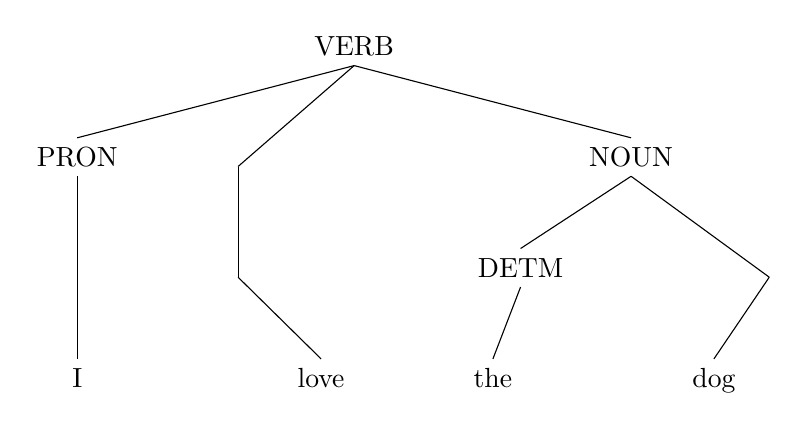
\begin{tikzpicture}[frontier/.style={distance from root=120pt}]
			\tikzset{sibling distance=40pt,level distance=40pt}
%			\tikzset{frontier/.style={distance from root=120pt}}
			\Tree[.VERB 
				[.PRON [ [.I ] ] ]
				[ [ [.\node[xshift=30pt]{love}; ] ] ]
				[.NOUN 
					[.\node[xshift=10pt]{DETM}; [.the ] ]
					[ [.\node[xshift=-20pt]{dog}; ] ]
				]
			]
		\end{tikzpicture}
	\end{figure}

	\begin{figure}
		\caption{Parse tree in constituency-based grammar}
		\label{parse tree in constituency-based grammar}
		\centering
		\Tree[.S
			[.NP [.PRON [.I ] ] ]
			[.VP [.VERB [.love ] ] [.NP [.DETM [.the ] ] [.NOUN [.dog  ] ] ] ]
		]
	\end{figure}

	\todo{fix graphs}
	
	Figure \ref{parse tree in dependency-based grammar} shows a sentence (`I love the dog') parsed into a dependency tree. Each node in the tree directly maps to a word in the sentence. Figure \ref{parse tree in constituency-based grammar} shows the same sentence in constituency tree format. Dependency grammars can be more useful in some circumstances because of their simpler nature - however, constituency grammars (or `phrase structure grammars') contain a lot more information about the phrase structure of the sentence, and so are better for the translation process. As such, \textit{yod}'s sentence input is given in constituency tree format.
	
	The tree input is represented as a JSON file, with properties of the object representing roots of subtrees of the current node. An input must be a single constituent of the tree, meaning the root must be a single node; the translation process can act on any node of the tree. The terminal nodes are represented by an object containing a \texttt{word} property which represents the English lemma of the word to be translated. This value is necessarily not inflected due to the fact that the lemma is needed to get a translation from the lexicon, and getting the lemma from an inflected English word is not necessarily a trivial task. Thus, preparing a sentence into the structure required by \textit{yod} requires a bit of manual editing, or a tool designed to use natural language processing to convert English sentences into this format. The JSON format was chosen over other forms of serialisation largely to allow for easy hand editing as well as compatibility with other software.
	
	The object which represents a terminal node also has a property which is a list of `tags' which represent different grammatical categories. This allows grammatical information to be carried through to the translation process, and allows for the possibility of morphological changes to be applied to generated words based on their grammatical categories. 
	
	The part of speech of the terminal node is represented by the key of its parent. When loading in a phrase from a JSON object, this information as well as all the information contained in the node is used to construct a logical representation of the sentence.
	
	This logical representation depends on the exact structure of the grammar required. \textit{yod} allows users to specify their own phrase structure grammar, as a full grammar of English would be too complicated for a user to be able to parse their sentences into, hindering the ease of use of the library. Allowing for custom grammars also allows users to devise more complex and unique languages - for example, if a writer wanted to create an alien language which lacked verbs, an English constituent grammar would not be sufficient. More complicated and unusual sentence structures can be permitted through a data-driven approach to creating a grammar. The grammar object should be thought of as representing the generated language's grammar, rather than an English grammar.
	
	Grammars are also serialised and deserialised as JSON objects or files containing JSON objects. These objects have a very simple structure: the object contains a key called \texttt{rules} which then contains a key for each non-terminal constituent in the grammar. For each of these constituents, there is a list of phrases that it can be expanded to. Each of these phrases consists of a list of constituents, terminal or otherwise, which is ordered such that when a sentence is translated, the elements of the phrase will be appended to the final sentence in that order.
	
	For phrases which contain multiple of the same constituent - for example, a compound noun phrase could be represented as \texttt{NOUN NOUN}, it is necessary to indicate the order in which these constituents are represented in order to distinguish the two nouns from each other when later translating the phrase. To accomplish this, duplicate constituents in phrases are marked with numbers; a compound noun in this form is represented as \texttt{NOUN-1 NOUN-2}.
	
	The last addition to the phrase structure grammar file is not necessarily a part of the grammar itself but instead an instruction on how to construct certain phrases in the language. This property is a list of rules which should be `compounded'. When the final translated sentence is constructed, a space is added between each constituent. If a rule is set to be compounded, however, the constituents of the rule will be concatenated without a space between them. A good example of this type of rule is the English language, where noun-noun compounds are frequently created by taking two nouns and concatenating them without a space: $fire + place \rightarrow fireplace$, $wrist + watch \rightarrow wristwatch$.

	An example phrase structure grammar which can be used to translate moderately complex English sentences is shown in figure \ref{example phrase structure grammar}.
	
	\begin{figure}
		\caption{Example phrase structure grammar}
		\label{example phrase structure grammar}
		\begin{tcolorbox}
			\begin{lstlisting}[breaklines=true,tabsize=2]
{
	"rules": {
		"S": ["NP VP", "S-1 CONJ S-2", "INTJ S"],
		"NP": ["PRON", "NN", "DETM NN", "NP PP", "NP RC", "PS NN"],
		"VP": ["VERB", "VERB NP", "VERB ADJC", "VERB PP", "VERB ADVB", "VERB PRON"],
		"PP": ["PREP NP"],
			"RC": ["RLTV VP"],
		"NN": ["NOUN", "ADJC NN", "CN"],
		"CN": ["NOUN CN", "NOUN-1 NOUN-2"],
		"PS": ["NOUN", "PRON"]
	},
	"compound": {
		"NN": ["ADJC NN"],
		"CN": ["NOUN-1 NOUN-2"]
	}
}
			\end{lstlisting}
		\end{tcolorbox}
	\end{figure}
	
	\section{Inflection}
   
   \printbibliography
\end{document}
